\documentclass[12pt, a4paper]{article}
%\usepackage{natbib}
\usepackage{cite}
\usepackage{amsmath,amssymb,amsfonts}
\usepackage{algorithmic}
\usepackage{graphicx}
\usepackage{textcomp}
\usepackage{xcolor}
\usepackage[inkscapeformat=pdf]{svg}
\usepackage[inline]{enumitem}
\usepackage[hidelinks]{hyperref}

\usepackage{myacronyms}
\usepackage{listings}
\usepackage{todonotes}
\newcommand{\note}[3]{\todo[inline,linecolor=#1,backgroundcolor=#1!25,bordercolor=#1]{\textbf{#2:} #3}}
\newcommand{\angela}[1]{\note{blue}{Angela}{#1}}

\newenvironment{inlinelist}{\begin{enumerate*}[label=\emph{(\roman*)}]}{\end{enumerate*}}

\usepackage{cleveref}

\begin{document}

%\title{Towards aggregate operating systems with Aggregate Computing}
%\title{Towards collective systems with Aggregate Computing}
\title{Towards collective operating systems through Aggregate Computing}
%\title{Towards collective operative environments with Aggregate Computing}
\author{Angela Cortecchia}
\date{\today}
\maketitle
%
%\setlength{\parindent}{0em}
%\setlength{\parskip}{1em}

% ----------------------------------------
\section{State of the art}
\label{sec:state-of-the-art}
% Esporre sinteticamente lo “stato dell’arte” relativamente al tema di ricerca prescelto,
% con le indicazioni bibliografiche essenziali.
% Se il progetto fa parte di una ricerca più ampia, evidenziare in modo specifico l’attività specifica che ci si propone di svolgere.
% Inserire inoltre gli elementi essenziali utili a dimostrare la coerenza del tema di ricerca prescelto con il percorso di
% formazione e le esperienze pregresse.
%\paragraph{Collective Adaptive Systems}
\sloppypar
\paragraph{Collective Adaptive Systems and Macroprogramming.}
\ac{cas} are systems composed of multiple autonomous entities,
including devices, sensors, and actuators, which interact locally to achieve a shared global objective~\cite{ferscha2015}.
%
These systems are designed to adapt to dynamic changes in the environment, system requirements, or operational conditions.
%
\ac{cas} are commonly employed in \ac{cps} applications where devices collaborate to monitor and control a
physical environment or to provide services to users.

Managing a single device in a distributed system presents several challenges,
such as \textbf{scalability}, \textbf{device heterogeneity},
\textbf{resource constraints}, and the need to adapt to \textbf{dynamic changes}.
%
Transitioning from a \emph{device-centric} approach,
where the collective is not the abstraction target,
to an \emph{aggregate-centric} approach can lead to various advantages, like
\begin{inlinelist}
    \item distributed intelligence,
    \item resource pooling,
    \item adaptability, and
    \item robustness.
\end{inlinelist}
%
The mentioned challenges can be addressed by using \emph{macroprogramming}.

\emph{Macroprogramming}~\cite{casadei2023} refers
to expressing the macroscopic behavior of a system through a single program using
macro-level abstractions.
%
This approach captures system-level behavior while abstracting individual component interactions.
%
Macroprogramming has been used in different contexts like \ac{wsn}~\cite{1440891}, \ac{iot} applications~\cite{noor19,mizzi18} and swarm robotics~\cite{buzz}.

\sloppypar
\paragraph{Self-organization and Field Calculus.}

Coordination models propose that interaction among multiple independent and autonomous software systems can be designed
orthogonally to pure computation, conceptualized as a shared data space.
%
Over time,
various approaches like \textit{Linda}~\cite{ViroliCoordination2012} and \textit{MARS}~\cite{mars} have emerged,
focusing on centralized local components rather than system distribution.
%
Key challenges in distributed systems include openness to environmental changes, large-scale agent coordination,
and intrinsic adaptiveness to ensure system resilience.
%
Addressing these challenges requires a \emph{self-organization and -coordination} approach,
managing logical interactions to
ensure global and robust coordination behavior.

To facilitate self-organization in complex environments, the \emph{coordination field} concept was introduced as a
navigational tool for agents.
%
The tuple-based middleware \textit{TOTA} (Tuples On The Air)~\cite{tota} supports field-based coordination in pervasive
computing applications.
%
Studies on distributed intelligent systems proposed computational fields for managing space-time
computing models, promoting higher abstractions of spatial collective adaptive systems~\cite{JLAMP2019}.

\ac{fc}~\cite{TOCL2019} emerged as a foundational model for coordinating computational devices in physical environments.
%
\ac{fc} was introduced as minimal core calculus with the aim of capturing the fundaments that make use of computational fields:
functions over and with fields, their evolution over time and the construction of field of values from neighbors.
%
It specifies aggregate system behavior through a dynamic network of directly communicating devices,
using functional compositions of operators manipulating computational fields.
%
Local specifications involve asynchronous computational rounds with three phases:
\begin{inlinelist}
    \item \emph{context building},
    \item \emph{program execution}, and
    \item \emph{export sharing}.
\end{inlinelist}
%
Globally,
\ac{fc} aligns individual device behavior with the network's overarching behavior,
specifying mappings for each device's computation round at space-time events.

\sloppypar
\paragraph{Aggregate Computing/Programming.}
\ac{ap} (or \ac{ac})~\cite{CASADEI2019252} is a functional macroprogramming approach for the compositional development
of self-adaptive \ac{iot} services,
based on the abstractions of \ac{fc}~\cite{MAMEIZL04}.

\ac{ac} programs the behavior of a distributed system by defining interactions among devices as a whole,
rather than individual device behavior,
shifting the fundamental computation unit from a single device to a collaborative group of devices.
%
This structure supports the specification, analysis, simulation,
and runtime execution of \emph{collective} or \emph{aggregate} services,
independently of specific \ac{iot} architectures~\cite{FI2020-pulverization}.
%
The paradigm has three key traits:
\begin{inlinelist}
    \item \emph{global stance with global-to-local mapping}, where the target of system design is the entire distributed \ac{iot} ecosystem,
    \item \emph{service compositionality}, describing rich collective services through the functional composition of simpler services,
    \item \emph{abstraction}, enabling adaptivity by abstracting from low-level details.
\end{inlinelist}
%
These attributes are crucial in both the \emph{design phase},
allowing concise and declarative articulation of complex solutions,
and the \emph{operational phase},
providing flexibility in execution specifics and deployment strategies.
%
Each device of the system locally evaluates the program at a certain frequency,
and communicates with neighboring devices when needed.

\sloppypar
\paragraph{Aggregate Processes.}

To address the challenges of managing multiple concurrent aggregate operations in a distributed environment,
a system has been developed for managing \emph{aggregate processes}~\cite{aggregate-processes} based on \ac{fc}.
%
Aggregate processes are concurrent field computations
whose execution and interactions are sustained by a dynamic team of devices,
and whose spatial region can opportunistically change over time.
%
This concept captures aggregate behavior, dynamicity and context orientation and intrinsic resiliency;
and as perks, it offers to limit the consumption of computational resources,
maintain a good quality of service,
and enhance the dynamics of distributed computations.

These types of processes differ from the concentrated ones.
%
In particular, there are specific issues that arise in the aggregate approach rather than the traditional one.
%
For example, managing process interruptions, determining the owner of a process and the resources it can access,
or understanding what it means to send a signal to a process.


\sloppypar
\paragraph{Tools for Aggregate Computing.}

Different tools have been developed to support the \ac{ac} paradigm,
each with its own characteristics and target devices.

\emph{ScaFi (Scala Fields)}\cite{scafi} is a Scala-based framework for aggregate programming,
it provides a \ac{dsl}, libraries, a simulation environment with a GUI,
integrated with the Alchemist simulator~\cite{PianiniJOS2013},
and an actor-based runtime for the development of aggregate computing-based systems.
%
ScaFi is capable of running aggregate programs on the \ac{jvm} and also on web browser thanks to the ScaFi Web tool~\cite{Coordination2021-scafiweb},
which allows the rapid prototyping of aggregate programs.

\emph{Protelis}~\cite{PianiniSAC2015} is a functional programming language that implements a higher-order version of the \ac{fc},
exposed through a C-like syntax,
enabling the construction of widely reusable components of aggregate systems.
%
It also provides various domain-specific APIs that are interoperable with Java, the Protelis-Lang~\cite{SASO2017-protelislang}.
%
Being based on \emph{Xtext},
it necessarily requires a \ac{jvm} to run,
which limits the heterogeneity of devices that can be used in the system.

\emph{FCPP}~\cite{DBLP:journals/scp/AudritoT24} is an implementation of the \ac{fc} as a C++ library,
with tools for simulations of distributed systems.
%
It allows running aggregate programs on low computational capacity devices.
%
However,
its syntax is less ergonomic compared to other languages,
making it unlikely to reach a mainstream developer audience.

\emph{Collektive} is a prototype \ac{dsl} for aggregate computing that extends the \ac{fc} with the \ac{xc}~\cite{AudritoCDSV24},
providing a more expressive language for the development of aggregate systems.
%
This language is more modern and has a user-friendly syntax compared to FCPP and Protelis;
moreover, it is natively multi-platform,
allowing the development of aggregate systems on different devices.

\subsection{Coherence with my previous experiences}
\label{subsec:coherence-with-the-educational-path}

The research project proposed can be seen as an extension of the research activities
carried out with my Master's degree final year and thesis.
%
During the Master's degree,
the exploration of \ac{fc} and \ac{ac} began as a project of the course ``Pervasive Computing''.
%
My project's colleagues and I developed a reimplementation of aggregate computing in Rust,
more specifically the core of the engine inherent to the \ac{fc}.
%
In addition to the development of the engine in Rust,
we also developed a version in Scala 3 of the engine's core that was already implemented in Scala 2,
which is the language used by the ScaFi project.
%
This work provided me with a good foundation in the field of \ac{ac} and \ac{fc}.

The Master's thesis was also focused on the \ac{ac} paradigm.
%
The goal of the thesis was to expand the work done on the Collektive \ac{dsl} previously developed,
by adding the constructs of the \ac{xc} calculus to the language.
%
At the end of the thesis, a prototype of the language was ready and tested on simple case study,
showing the potential of the language in the development of \ac{ac} applications.
%
The thesis therefore helped me to deepen my knowledge of the \ac{ac} paradigm and to understand the potential
of the language in the development of \ac{ac} applications.

During the development of the Master's degree,
I had the opportunity to apply for a research grant that was awarded to me from the \emph{Consortium GARR},
the Italian ``Group for Research Networks Harmonisation'',
and it is currently ongoing.
%
The research grant has the focus on the extension of the work done on the Collektive \ac{dsl},
by creating a standard library of functions that can be used in the development of \ac{ac} applications,
and various demos to show the functionalities of the language.

This experience has allowed me to submit a paper to the \emph{IEEE International Conference on Autonomic Computing and Self-Organizing Systems} (ACSOS 2024),
which is currently under review,
about a generalization of the \emph{Vascular Morphogenesis Controller} (VMC)~\cite{ZahadatHS17} algorithm using the \ac{ac} paradigm.
%
Another paper is currently under submission to the \emph{International Symposium on Distributed Simulation and Real Time Applications} (DS-RT 2024).
%
It is about the development of an architecture and prototype
for monitoring distributed simulations of distributed systems,
where my contribution consists of the development of the simulations used in the evaluation of the architecture,
done using Collektive.

% ----------------------------------------
\section{Project description}
\label{sec:project-description}

%\sloppypar
\subsection{Motivation.}
\label{subsec:motivation.}

Typical applications of aggregate computing implement and execute a single, albeit complex, algorithm.
%
However,
there are scenarios where these aggregated algorithms need to be added, removed,
or manipulated at runtime without affecting the others.
%
For example,
in a crowd management situation where people are directed to move in a certain direction,
congestion might occur,
requiring law enforcement to alter the movement of a portion of the crowd.

This concept parallels how modern operating systems manage processes, but in space and time.
%
To achieve similar functionalities in the realm of aggregate computing,
it is necessary to advance towards the development of \emph{aggregate operating systems}.
%
%To coordinate \ac{cas} scenarios in an efficient and effective way,
%there is the need to push the abstraction boundaries further than actual existing approaches.
%
%This can be achieved by developing a new generation of self-organizing collective systems.
%
These systems, in fact,
face concerns akin to those of ``concentrated'' operating system,
such as the management of devices, users, groups and relative permissions, and signals;
but in a distributed environment in which these concepts assume a different meaning
entailing space and time.
%
Additionally,
\acp{cas} are usually composed of heterogeneous devices,
meaning that the system must be able to,
simultaneously,
abstract away their differences and manage their specificities.
%
%The goal of creating a new generation of operating systems based on \emph{collective operating environment}
%for opportunistic mobile applications and services is well known in literature,
%but few studies have been conducted to effectively develop such systems.
%%
%Managing multiple concurrent aggregate operations -- where the execution is distributed over space and time
%-- poses a significant challenge that is increasingly necessary.

\subsection{Idea.}
\label{subsec:idea.}

\begin{figure}
    \centering
    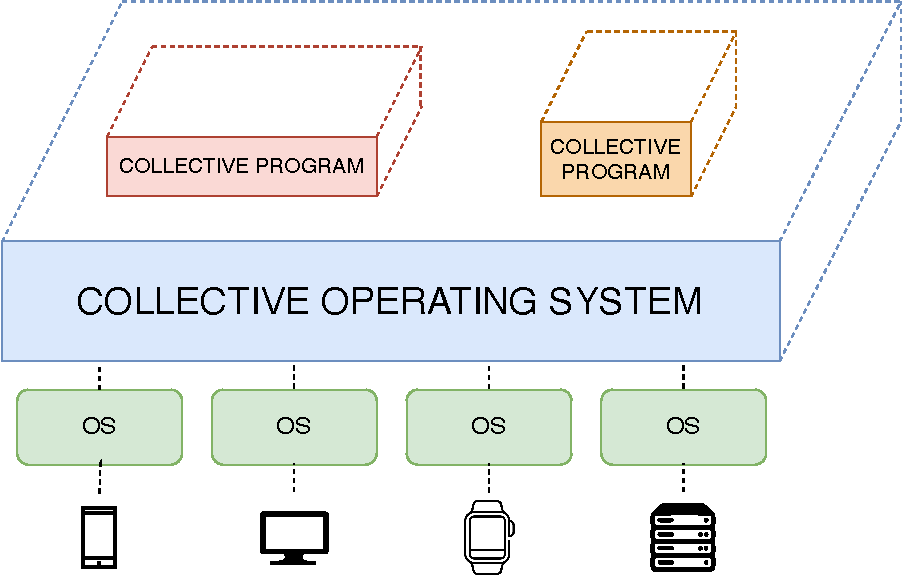
\includegraphics[width=0.8\textwidth]{figures/system}
    \caption{
        High-level view of the system.
        The collective operating system is seen as a middleware that manages the different aggregate programs and the devices
        of different types.
    }\label{fig:system}
\end{figure}

\begin{figure}
    \centering
    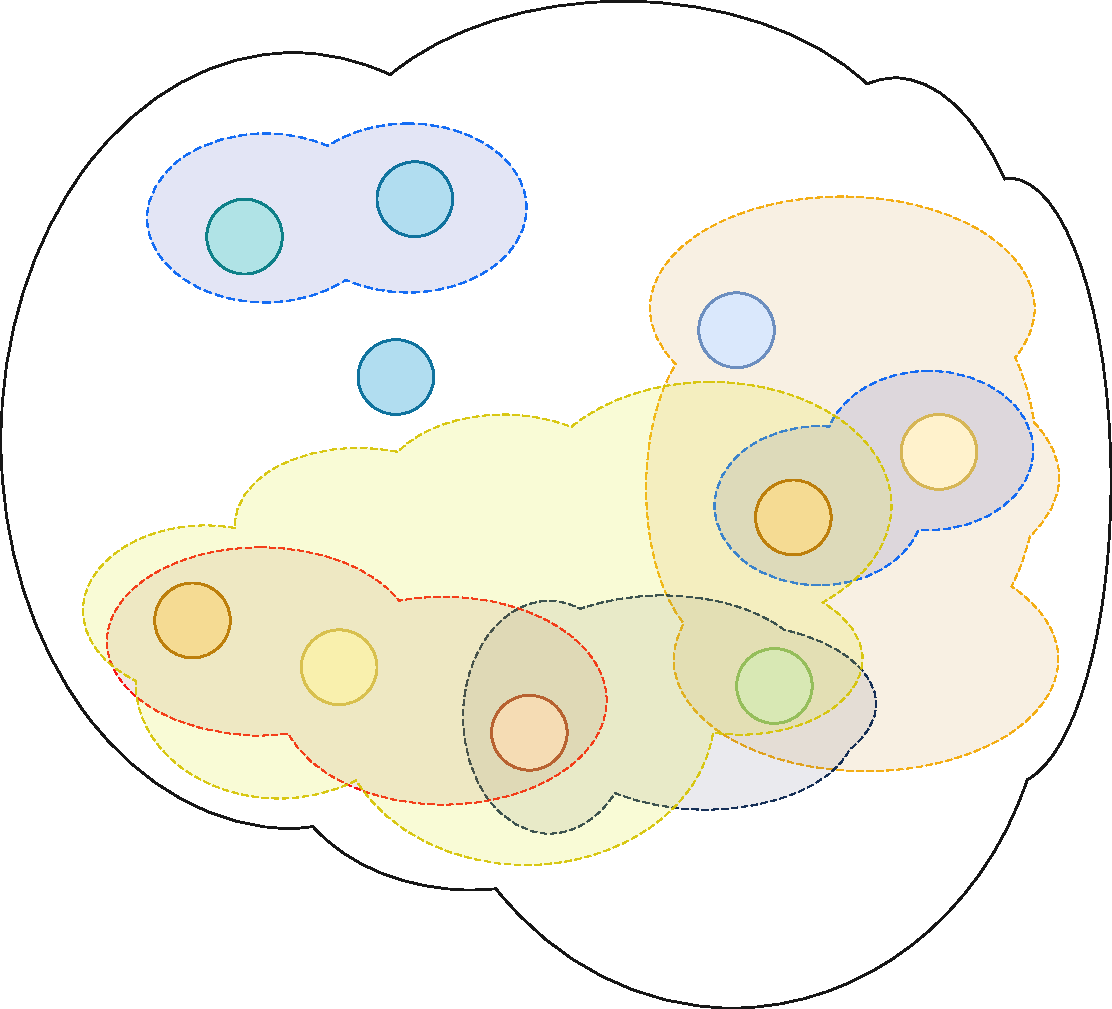
\includegraphics[width=0.99\textwidth]{figures/processes}
    \caption{
        Aggregate processes executed on a collective operating system.
        Solid circumferences represent devices, their internal color indicates the device kind
        (same color, same kind).
        The space delimited by the solid black line indicates the region of the space where the
        operating system is active.
        Dashed zones are aggregate processes,
        the same color indicates the same process.
        Notice that devices may participate in one, none, or multiple processes.
        Also, differently than the current proposal for aggregate processes,
        with the proposed approaches the same process can be non-contiguous in space-time.
    }\label{fig:processes}
\end{figure}

%It follows that the concept of developing a new infrastructure that allows the use of multiple aggregated processes within
%a similar aggregate operating system naturally arises.
%
The general idea of the project is conveyed graphically by
\Cref{fig:system} and \Cref{fig:processes}.
%
\Cref{fig:system} shows a high-level view of the system,
where the collective operating system works as middleware between the different aggregate programs and the devices where they run.
%
From another perspective,
\Cref{fig:processes} shows collective processes that execute over the shared operating system,
involving different sub-portions of the space-time.
%
Each process can be executed on different devices and a device can execute different processes,
so it is possible to have an overlap of processes on the devices.
%
Note that, differently than the current aggregate processes~\cite{EAAI2020-processes},
through the proposed approach
the shared operating system permits processes which are non-contiguous in space.


\subsection{Research goals and challenges}
\label{subsec:research-goals-and-challenges}

Realising a similar system requires an understanding of the meaning of various concepts when they are tied to space and time.

\paragraph{Users and permissions.}
In classic operating systems exists a subdivision of users and groups,
and access to resources and services is based on the user's role relative to the context in which they are located.
%
In an aggregate or collective context,
at the moment,
there is no clear definition if what a user (or group) is and how to manage its permissions inside the collective system.
%
For example,
in a crowd management scenario,
there are more types of users: the people that are part of the crowd and the law enforcement that cam manage the crowd.
%
Clearly,
the law enforcement has more permissions than the people in the crowd and can execute different actions.
%

\paragraph{Signals and interrupts.}
Similarly, the concept of interrupt and signal cannot be simply inherited from the traditional operating systems,
and needs rethinking.
%
Signals are an analog problem as permissions, it must be clear who sends a signal because it can
change the behavior of the recipient process.
%
It must be possible to send a signal of termination or kill to a process,
without affecting the other processes,
and it must be defined who can effectively send a certain kind of signal to processes;
this is therefore related to the concept of permissions.
%
Moreover,
it must be investigated what a pause or continue or kill signal means in an aggregate environment.
%
For instance,
in the aggregate approach termination is managed collectively.
%
However,
there may be situations where a single device decides to terminate processes or where a process using shared
resources loses the right to use them during execution,
introducing a distributed consensus problem.

Using the example of the crowd management scenario,
there may be situations of crowd sensing or crowd steering where law enforcement realizes that too many people are gathering.
%
Depending on the situation,
third-party entities that are allowed to send certain kinds of signals can decide to interrupt the crowd-management process.

The need of sending signals to processes while they are running,
establish the need of a mechanism to enable the change of the behavior of the system at runtime.

\paragraph{Intra-process communication.}
Communication between processes in different regions of space is another issue that needs to be addressed.
%
For example,
in a crowd steering and crowd tracking scenario,
there are different processes that need to communicate between them to manage the crowd.
%
A process managing the crowd steering needs to communicate with the process that is managing the crowd tracking,
to understand where the people are and how to move them.

Moreover, intra-process communication,
mediated by shared memory spaces or files in traditional systems,
is not applicable as-is when processes are inherently distributed,
so further research is needed from this point of view.

\paragraph{Distributed sensors and actuators.}
Another challenge is the management of distributed sensors and actuators.
%
Combining the capabilities of multiple devices to achieve a common observation as a single entity or logical resource,
can lead to a more abstract and high-level programming approach,
and to involve heterogeneous devices in the system.
%
In the crowd management scenario,
there may be involved various sensors or devices that observe the crowd,
sending data to the system to manage the crowd.
%
The system should see data received from different devices as it was a single entity,
allowing for a more abstract and high-level programming approach.
\\

The proposed research project therefore aims to investigate the development of \emph{collective operating systems},
based on the \ac{ac} paradigm.
%
The paradigm itself of \ac{ac} also offers consistency and resilience to failures,
and the possibility to adapt to \emph{dynamic} changes in the environment.

\subsubsection{Example applications.}
An application instance is the management of a drone fleet in a surveillance scenario,
in which drones collaborate to monitor an area.
%
From the point of view of the application designer,
however,
the whole fleet is seen as a single entity,
and the objects in the field of view of each drone constitute a single ``collective sensor'',
realizing a form of ``sensor fusion''~\cite{sasiadek2002sensor} at the application level.

Other examples are in the management of a smart city,
where the system has to manage the data of the city and the users.
%
To avoid light pollution,
it could be useful to manage the lighting of the city based on the presence of people in the streets,
or to manage the traffic lights based on the presence of cars in the streets.
%
In a crowd management scenario,
the system can manage the movement of the people to avoid congestion,
eventually having the law enforcement to manage the crowd,
sending signals to the system to change the direction of the people.

% ----------------------------------------
\section{Expected results}
\label{sec:expected-results}

As results of the proposed research project,
it is expected to bring
\begin{inlinelist}
    \item a contribution to the advancement of scientific and technological knowledge in the field of \ac{ac} and \ac{cas},
    \item a formal model of how it should work,
    \item a prototype of the system that is able to manage in a simple and effective way some of the problems that arise in a collective environment.
\end{inlinelist}
%
For instance,
one of the problems presented involves communication between ships in the Kiel Canal
and the amount of data that they can exchange depending on the type of communication available.
%
Specifically,
the farther apart the ships are,
the fewer data they can automatically exchange.
%
Currently,
this issue remains unresolved in an effective manner.
%
Therefore,
it is believed that through \ac{ac},
and particularly through the use of \ac{xc},
a contribution can be made towards solving this problem.

As a long-term vision,
the system will be able to manage many devices in a collective environment,
where the devices can be heterogeneous and can change over time.
%
Some of the application scenarios where the system can be used are
\begin{inlinelist}
    \item \emph{smart cities},
    \item \emph{swarm scenarios},
    \item \emph{crowd management},
    \item \emph{morphogenesis},
    \item \emph{autonomous vehicles},
    \item \emph{surveillance}.
\end{inlinelist}

% ----------------------------------------
\section{Subdivision of the project and timeline}
\label{sec:subdivision-of-the-project-and-timeline}

\begin{figure}
    \centering
    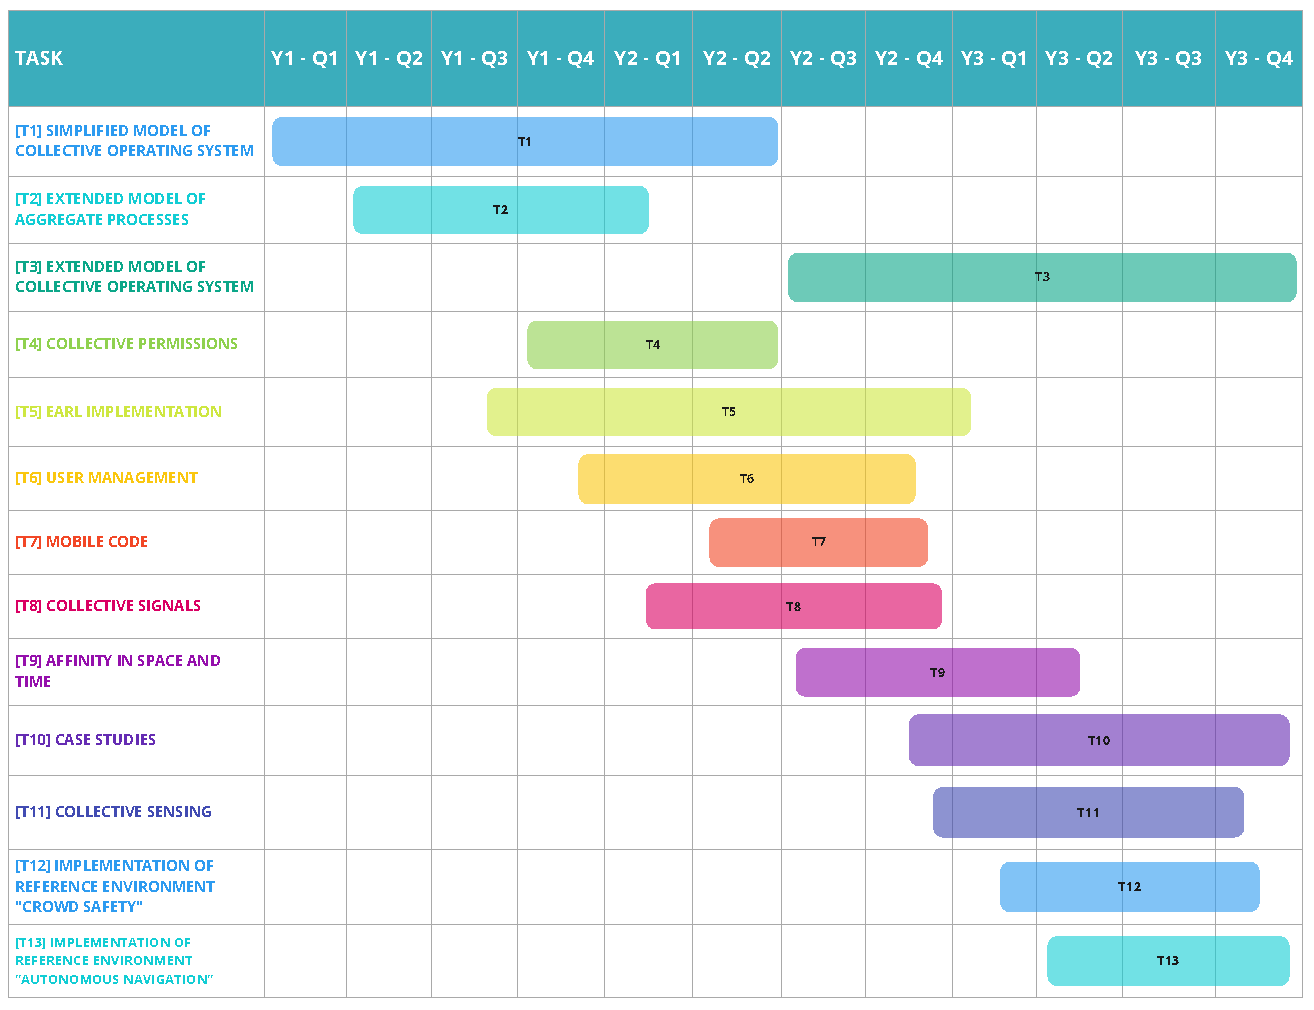
\includegraphics[width=0.99\textwidth]{figures/timeline}
    \caption{Hypothetical timeline of the three years of the project.
        Years are subdivided in quarters, Q1 is from January to March,
        Q2 is from April to June, Q3 is from July to September, and Q4 is from October to December.
    }\label{fig:timeline}
\end{figure}

In the \Cref{fig:timeline} is shown a hypothetical timeline with tasks of the three years of the project,
where each year is subdivided into quarters.

\sloppypar
\paragraph{First year}
In the first year of the project,
it is essential to thoroughly investigate the state of the art and create a simplified model of how the new system should work.
%
The simplified model (identified as \texttt{T1})
will include the definition of the main interconnected concepts of the system,
such as the implementation of the aggregate processes,
the management of permissions and the collective sensing of external devices.
%
Following this,
the actual development process begins with the prototype implementation (\texttt{T3}) in the target language Collektive.
%
At the end of the first year,
there will be enough foundations to start the development of the system in a use case scenario.
%
The use case, identified as \texttt{T4},
will be relevant to the crowd safety scenario,
including crowd steering, sensing, and tracking.

\sloppypar
\paragraph{Second year}
The second year of the project will be focused on completing the simplified model of the system (\texttt{T1}),
leading to the development of the extended model (\texttt{T2}),
that includes the management of users or groups, signals and interrupts, and intra-process communication.
%
Throughout the year,
the focus will be on continuing the development of the prototype (\texttt{T3}),
expanding on the concepts investigated in the first year,
and incorporating features such as runtime aggregate programs injection.
%
Eventually,
when considering the international research stay,
the plan is to establish contacts with companies or research groups that possess the necessary hardware to test the system.
%
Towards the end of this period,
the first use case (\texttt{T4}) will be implemented and tested in a simulated environment,
leaving space to the implementation of the second use case inherent to the autonomous navigation scenario (\texttt{T5}).

\sloppypar
\paragraph{Third year}
In the third and final year of the project,
the extended model of the system will be completed (\texttt{T2}), alongside the development of the prototype (\texttt{T3})
and the implementation of the third use case scenario mentioned before (\texttt{T5}).

% ----------------------------------------
\section{Proposed evaluation criteria}\label{sec:proposed-evaluation-criteria}

\sloppypar
\paragraph{Qualitative.}
Qualitative evaluation will be based on the development of open-source software capable of being used in simulations and real-world
environments on heterogeneous devices.
%
The degree of qualitative success will depend on the features implemented among those previously discussed.

\sloppypar
\paragraph{Quantitative.}
Quantitative analysis can be assessed through the effective functioning of the system in simulated scenarios,
which are expected to be obtained relatively soon.
%
However,
field-testing is more challenging due to the need for specific hardware.
%
In this regard,
the possibility of securing a partnership for an international research stay during the PhD program will be pursued,
where appropriate hardware is available to test the project.

\sloppypar
\paragraph{Scientific contribution.}
In terms of scientific results and dissemination,
a couple of papers have already been submitted and are currently under review.
%
The goal is to produce and submit papers to approximately one or two conferences per year and to have several articles submitted to journals.
%
The focus will be on the key communities, which have as topic ``self-organizing systems'',
such as \emph{ACSOS}\footnote{\url{https://acsos.github.io}} or \emph{SEAMS}\footnote{\url{https://conf.researchr.org/home/seams-2025}},
or even journals such as \emph{ACM TAAS}\footnote{\url{https://dl.acm.org/journal/taas}}.

% ----------------------------------------
\bibliographystyle{IEEEtran}
\bibliography{bibliography}

\end{document}
